%Input preamble
%Standard HelperFile at the CEHD
%Style
\documentclass[11pt]{article}
\usepackage[top=1in, bottom=1in, left=1in, right=1in]{geometry}
\parindent 22pt

%Packages
\usepackage{adjustbox}
\usepackage{amsmath}
\usepackage{amsfonts}
\usepackage{amssymb}
\usepackage{bm}
\usepackage[table]{xcolor}
\usepackage{tabu}
\usepackage{makecell}
\usepackage{longtable}
\usepackage{multirow}
\usepackage[normalem]{ulem}
\usepackage{etoolbox}
\usepackage{graphicx}
\usepackage{tabularx}
\usepackage{ragged2e} 
\usepackage{booktabs}
\usepackage{caption}
\usepackage[none]{hyphenat}
\usepackage{fixltx2e}
\usepackage{threeparttablex}
\usepackage[capposition=top]{floatrow}
\usepackage{subcaption}
\usepackage{pdfpages}
\usepackage{pdflscape}
\usepackage{natbib}
\definecolor{maroon}{HTML}{990012}
\usepackage[colorlinks=true,linkcolor=maroon,citecolor=maroon]{hyperref}
%\doublespacing

%Functions
\DeclareMathOperator{\cov}{Cov}
\DeclareMathOperator{\var}{Var}
\DeclareMathOperator{\plim}{plim}

%Math Environments
\newtheorem{theorem}{Theorem}
\newtheorem{assumption}[theorem]{Assumption}
\newtheorem{condition}[theorem]{Condition}
\newtheorem{example}[theorem]{Example}
\newtheorem{exercise}[theorem]{Exercise}
\newtheorem{remark}[theorem]{Remark}
\newtheorem{claim}[theorem]{Claim}
\newtheorem{lemma}[theorem]{Lemma}
\newtheorem{definition}[theorem]{Definition}
\newtheorem{hypothesis}[theorem]{Hypothesis}
\newtheorem{property}[theorem]{Property}
\newenvironment{proof}[1][Proof]{\noindent\textbf{#1.} }{\ \rule{0.5em}{0.5em}}

\newcommand\independent{\protect\mathpalette{\protect\independenT}{\perp}}
\def\independenT#1#2{\mathrel{\rlap{$#1#2$}\mkern2mu{#1#2}}}
\newcommand{\overbar}[1]{\mkern 1.5mu\overline{\mkern-1.5mu#1\mkern-1.5mu}\mkern 1.5mu}
\newcommand{\equald}{\ensuremath{\overset{d}{=}}}

\renewcommand{\rothead}[2][60]{\makebox[9mm][c]{\rotatebox{#1}{\makecell[c]{#2}}}}
\newcommand{\mr}{\multirow}
\newcommand{\mc}{\multicolumn}

\begin{document}

\title{Factor Analysis}
\author{Jorge Luis Garc\'{i}a\thanks{Department of Economics, the University of Chicago (jorgelgarcia@uchicago.edu).} $^{,}$\thanks{I thank Sneha Elango, Tim Kautz, and Bradley Setzler for helpful comments.}}
\date{First Draft: May 29, 2014 \\ This Draft: \today}
\maketitle


\begin{abstract}
\noindent The objective of this document is to describe a step-by-step methodology to extract factors, or underlying latent variables, from a set of observed measures. Factor analysis is arbitrary by construction. Thus, I intend to provide the exact steps for factor analyzing a set of measures and elect a consistent way of being arbitrary. The theoretical fundamentals of this document come from \citet{gorsuch1983factor}. Although this author (or any other author) does not suggest any method over the other, I justify why the methods I elect are simple and transparent. Finally, I provide implementations in Python and Stata in separate files.
\end{abstract}

%Diagonal Factor Analysis
\section{Diagonal Factor Analysis} \label{section:dfa}
\subsection{Setting}
Let $v = 1, \ldots, V$ index the number of measures and $f = 1, \ldots, F$ the number of factors in the sets $\mathcal{V}, \mathcal{F}$, with cardinaliies $V$ and $F$, respectively. Let $n = 1, \ldots, I$ index the individuals observations in the set $\mathcal{I}$ with cardianlity $I$. $X_{iv}$ is \textit{observed} measure for individual $i$. It loads on the factors $F_{i1}, \ldots, F_{iF}$ and the factor loadings are the real numbers $w_{v1}, \ldots, w_{vF}$. Thus, the measurement system for individual $i$ is 
\begin{eqnarray}
X_{i1} &=& w_{11}F_{i1} + \cdots + w_{1F}F_{iF} + \eta_{i1} \nonumber \\
\vdots &=& \ddots \nonumber \\
X_{iV} &=& w_{V1}F_{i1} + \cdots + w_{VF}F_{iF} + \eta_{iV} \label{eq:system} \\
\end{eqnarray}

\noindent where $\eta_{iv}$ is measurement error in the measure $v$ of individual $i$ and satisfies the mean independence property, i.e. $\mathbb{E} \left( \eta_{iv} | F_{if}  \right) = 0$ for $f = 1, \ldots F$.\\
\indent We observe the LHS of \eqref{eq:system} as a set of measures and we do not observe the RHS. The objective of factor analysis is to recover $F_{i1}, \ldots, F_{iF}$, i.e. to recover a set of underlying scores defining the measures  $X_{i1}, \ldots, X_{iV}$. This with the objective of, for example, obtaining a reduction in the dimension of the problem at hand.\footnote{An example of this is \citet{bernal2011child}. They have a set of instruments shifting women's labor supply in the US. Given that welfare rules are the base of their instruments and the welfare system in the US is complex, the set of instruments is very wide and they face a ``many instruments problem'', i.e. 2SLS estimates are biased towards OLS estimates when the number of overidentifying instruments is large \citep[see][]{stock2002testing,andrews2007testing,hansen2008estimation,anderson2010asymptotic}. Thus, they factor analyze their set of instruments and argue that their 2SLS estimates are similar to LIML estimates, which correct the bias in 2SLS in the case of many instruments \citep[see][]{hansen2008estimation}.}
\subsection{Notation}
I define the basic notation throughout this document in the following lines. I do not assume that, in general, all the measures or all the factors or all the individuals are considered. That is a particular case when $n= N, f=F, v=V$ in some of the equations below, which are straightforward to recognize.\footnote{To ease matrix calculation and interpretation I use a subindex to indicate the dimensions of each matrix.}
\begin{enumerate}
\item Measures matrix (in deviation): \\
\noindent The data matrix containing $v$ measures for $n$ individuals \textit{in deviations from the mean} is $X_{nv}$ .
\item Measures matrix (standardized): \\
\noindent The data matrix containing $v$ measures for $n$ individuals \textit{in standardized form} is $Z_{nv}$.
\item Factor score matrix (standardized): \\
\noindent The factor score matrix containing $f$ common factor scores for $n$ individuals \textit{in standardized form} is $F_{nf}$.
\item Factor loadings matrix:\\
\noindent The factor loadings matrix containing the $v$ weights for $f$ factors ``to recover measures from factor scores'' (in a full components model in the absence of measurement error) is $P_{vf}$.
\noindent The factor loadings vector containing the $v$ loadings for $f$ factors is $P_{vf}$.  
\item Measurement error matrix:\\
\noindent The measurement error matrix containing $v$ error terms for $n$ individuals is $U_{nv}$.
\item Measurement error weights:\\
\noindent The measurement error weights containing the $v$ weights for $v$ equations is $D_{vv}$. In this document I assume that this matrix is equal to the identity matrix of size $v$, $I_{vv}$.
\item Matrix system:\\
\noindent The standardized measurement system for $n$ individuals, $v$ measures, and $f$ factors is
\begin{equation}
Z_{nv} = F_{nf} P'_{fv} + U_{nv} D'_{vv}.
\end{equation}
\item Covariance matrix of the measurement system (in deviation):\\
\begin{equation}
C_{vv} := \frac{1}{N} X'_{vn}X_{nv}.
\end{equation}
\item Correlation matrix of the measurement system (in deviation):\\
\begin{equation}
R_{vv} := S_{vv}^{-1} C_{vv} S_{vv}^{-1}. \label{eq:corrsysstd}
\end{equation}
\noindent where $S_{vv}^{-1}$ is a diagonal matrix and contains the standard deviation of measurement $v$ in entry $vv$. Importantly, $R_{vv} = \frac{1}{N} Z'_{vn}Z_{nv}$. Thus, $S_{vv}^{-1}$ allows to go from $X_{nv}$ to $Z_{nv}$. 
\end{enumerate}

\indent $U_{nv}$ could either be a factor that is dedicated to one measure or measurement error. These are indistinguishable from the perspective of the statistician who extracts factors. There is a simplifying procedure that allows us to ignore $U_{nv}$ in the context of Economics, and it is the following: (i) ignore the existence of $U_{nv}$ and assume the complete measurement system is correlated; (ii) extract the factors; (iii) consider the measurement error in measurement system as part of the system for which the factors are inputs. Concretely, a method extracts factor $F_{iv}$ for individual $i$ while the ``real'' factor is $\hat{F_{iv}} + \eta_{iv}$. A standard treatment of $F_{iv}$ as a variable with measurement error enables us to consider it in the context of regression analysis. This is why henceforth I consider the system
\begin{equation}
Z_{nv} = F_{nf} P'_{fv}.
\end{equation} 
\subsection{Residual Factor Analysis} \label{section:method}
\citet{gorsuch1983factor} calls my preferred method \textit{diagonal analysis}. Other literature names it triangular decomposition, sweep-out method, pivotal condensation, solid-staircase analysis, analytic factor analysis, maximal decomposition, or regression component analysis \citep[see][Chapter 2]{gorsuch1983factor}. In fact, maybe the last name is the one that makes the most sense because the method has as its basic ingredient a fundamental of regression analysis, residual matrices. Residual factor analysis sounds even fancier.\\
\indent These are the steps to extract the factor loadings of $F$ factors from the measurement system with $V$ measures from $N$ individuals. The method to obtaining the factor scores once the factor loadings are calculated is in Section \ref{sec:scores}, and the method to determining the number of factors to be extracted is discussed in Section \ref{section:nfactors}. 
\begin{enumerate}
\item Pick the first factor: elect one of the measures in the measurement system as the first factor. There are two possibilities for doing this:
\begin{enumerate}
\item Arbitrary: elect one measure with transparent meaning. In this case the objective is to have a well-known, meaningful measure as first factor.
\item Maximum correlation across the measurement system: (i) compute the covariance matrix of the measurement system and square each of its entries; (ii) compute the sum of all its columns; (iii) pick the measurement with the largest sum.  In this case the objective is to have the measure that correlates the most with the rest of the measurement system as first factor.
\end{enumerate}
\item Compute the factor loadings for the first factor: the factor loadings for the first factor are the correlation coefficients of the first factor with the variables in the measurement system. Naturally, the factor loading of the first factor with the measure that defines it is $1$. Denoting with lower case letters the entries of \eqref{eq:corrsysstd} the factor loadings for the first factor are defined as:
\begin{equation}
w_{11} := r_{11}, \ldots, w_{V1} := r_{V1}. 
\end{equation}
\noindent These loadings define $P_{V1}$, i.e. the vector stacking the $V$ loadings of factor 1.
\item Residualize the correlation matrix: obtain the correlation matrix of the measurement system after making it orthogonal to the first factor. Let $R_{vv}^{o1}$ correlation matrix of the measurement system after making it orthogonal to the first factor. Thus
\begin{equation}
R_{VV}^{o1} = R_{VV} - P_{V1} P'_{V1}. 
\end{equation}
\item Obtain a second factor: repeat steps 1 and 2. Usually, the second factor is going to be chosen based on criterion (b) in step 1 because after making the system orthogonal to the first factor it is difficult to interpret what the measures mean. 
\item Obtain factors $3, \ldots, F$: repeat the process making the measurement system orthogonal to factors 1 and 2 in order to obtain factor 3. Likewise, repeat the process making the system orthogonal to factors 1, 2, \ldots, F-1 to obtain factor $F$.  
\end{enumerate}

\subsection{Obtaining the Factor Scores} \label{sec:scores}
In the case when we have $N$ individuals, $V$ measures, and $F$ factors the measurement system is
\begin{equation}
Z_{NV} = F_{NF} P'_{FV}. \label{eq:sys}
\end{equation}

\noindent A simple manipulation of \eqref{eq:sys} leads to
\begin{equation}
F_{NF} = Z_{NV} P_{VF} \left( P'_{FV} P_{VF} \right)^{-1}, 
\end{equation}

\noindent which solves for the factor scores.
\subsection{How many Factors?} \label{section:nfactors}
\noindent I follow \citet{guttman1954some} and elect the lower bound of the number of factors based on a simple rule of thumb. The steps are the following.
\begin{enumerate}
\item Calculate the absolute value of the eigenvalues of the correlation matrix of the measurement system.
\item Count the number of eigenvalues greater or equal than one.
\item Define the lower bound of the number of factors as the number of eigenvalues greater than one.
\end{enumerate} 

\indent Once the lower bound is defined, as many eigenvalues as independent measures in the measurement system may be calculated. These are the inputs of the \textit{subjective scree test}. The scree test is an eye ball test of a scatter in which the abscissas are the factor numbers and the ordinates are their corresponding eigenvalues. The lower bound of the number of factors is the actual number of factors if the plot shows a very clear pattern differentiating the factors with eigenvalues greater or equal than one from the rest. In Figure \ref{fig:scree} the lower bound of the number of factors and the actual number of factors are the same according to my criterion because the factors with eigenvalues less than one follow a different pattern from the rest. 

\begin{figure}[H]
	\caption{A Scree Test where the Lower Bound and the Current Number of Factors Agree} \label{fig:scree}
  	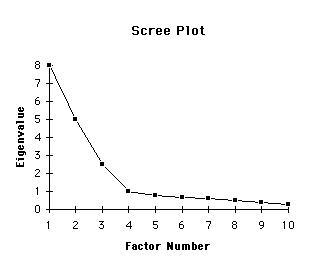
\includegraphics[width=2in, height=2in]{screetest.png}
\end{figure}
\subsection{Other Annotations}

\subsubsection{Correcting for Attrition}
\noindent It is very common for economists to correct for attrition. This is, to correct for the fact that some variables are not observed for certain individuals. A usual way to do it is to estimate a model predicting the probability of attrition based on observed characteristics. For example, if income is an outcome of interest and the researcher does not observe income for a subset of the sample but has observed characteristics for the complete sample, she can predict the probability of attrition. Then, she can use a method such as inverse probability weighting (IPW) to give greater relative weight to the observations that are more likely to have attrition \citep[see][]{wooldridge2007inverse}.\\
\indent Provided the estimated model predicts attrition, it is easy to consider an IPW scheme in which factors are extracted using the method in Section \ref{section:method} --it is sufficient to consider the IPW scheme when calculating the correlation matrices.

\subsubsection{Allowing for Correlated Factors} \label{section:correlated}
\noindent By construction, the method in Section \ref{section:method} does not allow factors to be correlated. Sometimes, however, economic theory or intuition suggest that two or more sets of measurements should be considered. It is possible to apply the process in Section \ref{section:method} to two different sets of measurements independently. If the first factor of the two sets of measurements are correlated, this procedure preserves the correlation between the two first factors. When extracting the rest of the factors for each set of measurement systems, one can make the system orthogonal to the first factor of both systems as in step 3. Thus, the first factors of the two systems will be correlated while the rest of the factors will not be correlated within or across measurement systems.\footnote{I thank Tim Kautz for pointing this out. His example is the following. Assume the researcher has two measurements systems: one for height and one for weight. It makes sense to allow correlation for the ``primary'' measures of height and weight, which would be the first factors in this case, because it is natural for height and weight to be correlated. Then, it is possible to make the rest of the systems orthogonal because the researcher is only willing to capture extra variation or information from the measures.}

%Rotating the Factors Analysis
\section{Why Rotation Makes sense and How to Go about it?} \label{section:rfa}
\noindent In Section \ref{section:correlated} I discuss how to allow for correlated factors. The procedure implies being certain about having two sets of measurement systems clearly devoted to factors of interest. For example, a measurement system could be devoted to ``weight'' and another to ``height''. The researcher arbitrarily chooses the measures with which she constructs the ``weight'' factor and the measures with which she constructs the ``height'' factor.\\
\indent It could be the case that the researcher does not want to take any stand on what the measurement systems are. This could happen for two reasons: (i) the researcher does not want to take arbitrary stands on what the dedicated measurement systems are; (ii) the researcher has no idea on what the dedicated measurement systems are.\\
\indent If this is the case, the alternative method is the following: (i) decide on a set of items composing the measurement system; (ii) set the number of factors (e.g.,  through a procedure like the one in  \ref{section:nfactors}); (iii) factor analyze the measures (e.g.,  through a procedure like the one in \ref{section:method}); (iv) rotate the factor axes to gain interpretability of the factors.\\
\indent The first three steps are clear: the researcher decides what the measurement system is, decides the number of factor she wants to use, and factor analyses the measures according to her preferred method. Rotation is convenient in this context. In general, after factor analyzing a set of measures, the output does not have an intuitive structure. Most items load on the first few factors that explain the greatest proportion of variance. Rotation is a linear transformation intending to give a ``simple structure'' to the factor system. In rough terms, it seeks a structure in which items load strongly on one factor and weakly in the rest of the factor.\footnote{\citet{abdi2003factor} explains the mathematical requirements for a structure to be simple and the intuition behind them.} This is the way in which the researcher may be able to associate each factor to an object of economic interest, ``height'', ``weight'', etc.\\ 



%\clearpage
\bibliographystyle{chicago}
\bibliography{BibtexFiles/Resources}
\clearpage

\end{document}